\chapter{methodisches Vorgehen}

%- Grundlagen sind notwendig zur Bewertung der Systeme
%- die exakte Definition der Anforderungen und des Ist-Standes ist Voraussetzung zur Bewertung
%- die Struktur der Untersuchung der systeme dient dem einheitlichen vergleich und der Nachvollziehbarkeit
%- konkret: aufbau ist wichtig  zur beurteilung der leistungsfähigkeit; Installation und Schnittstelle sollen aufzeigen, dass das system unter der definierten Umgebung lauffähig ist; Datenimport zeigt die integrationsfähigkeit; Verarbeitung als wesentlicher Punkt, neben Aufbau Voraussetzung für Leistung, ; Leistungstests als quelle zum Vergleich der leistung
%- Verweis auf bestehende vergleiche (literatur)

%Dan:
%du wirst bestimmt dinge finden wie "Benchmark von Datenbanken"
% und ich meine ein gis ist ja nur eine DB (mit effizienter Datenhaltung für geographische Figuren) mit erweiterten Funktionen im gis kontext
%zu bewertung von software/is würde ich auf softwaretechnik bücher verweisen ... die du verwenden kannst, um dir eine eigene Liste von  Bewertungskritierien für deinen Anwendungsfall zu erstellen

Das Thema "Untersuchung und Optimierung von verteilten geografischen Informationssystemen zur Verarbeitung agrartechnischer Kennzahlen" besteht aus vier Unteraufgaben:\\

\textbf{Untersuchung bestehender Frameworks anhand von Qualitätsmerkmalen}\\
Die erste Hälfte dieser Arbeit ist eine Softwareauswahl im Bereich der Datenverarbeitung.
Es handelt sich dabei nicht im Anwendersoftware, wodurch keine empirischen Studien der Benutzung der Frameworks durch Anwender und keine Kopplung mit der Unternehmensstruktur notwendig ist.
In diesem speziellen technischen Kontext sind wissenschaftliche Vorgehensweisen zur Softwareauswahl notwendig.
Dafür geeignet ist eine Nutzwertanalyse. % TODO: begründen warum nicht anderes Model
Darin soll mit Mitteln des Softwarequalitätsmanagement und allgemein Prinzipien der Softwareentwicklung eine nachvollziehbare, auch auf ähnliche Projekte übertragbare und wissenschaftlich korrekte Vorgehensweise erreicht werden.\\
% TODO: Übergang
Aus gegebenen Anforderungen\footnote{siehe \ref{Anforderungen}} sind Qualitätsmerkmale zu erstellen.
Davon ist die Mindestmenge welche zur Eignung eines Frameworks notwendig ist bzw. die notwendige  Qualität zu definieren.
Darauf aufbauend sind Qualitätsmetriken zu erstellen, welche die einzelnen Qualitäten messbar machen.
Eine Menge von scheinbar geeigneten Frameworks ist anhand der definierten Metriken zu untersuchen.
%TODO: auf Listen der Community zurückgreifen
Dabei sind jedoch nur die wesentlichen Qualitäten zu untersuchen.
Aus bekannten GIS Frameworks werden vielversprechende ausgewählt und somit die Menge der zu untersuchenden Frameworks erstellt.
Diese Vorauswahl erfolgt anhand der Tabelle \glqq Table of free systems especially for spatial data processing\grqq\ in \cite{website:wiki-spatialdatabase}.
Wikpedia dient dabei als Quelle, da diese Website von Arbeitnehmern genutzt wird und somit diese Community die Tabelle aktuell und ausreichend vollständig hält.
Dies ist in der Aufrufstatistik begründet, welche in Abbildung \ref{fig:wiki-usage-spatialdatabase} dargestellt ist.
\begin{figure}
\centering
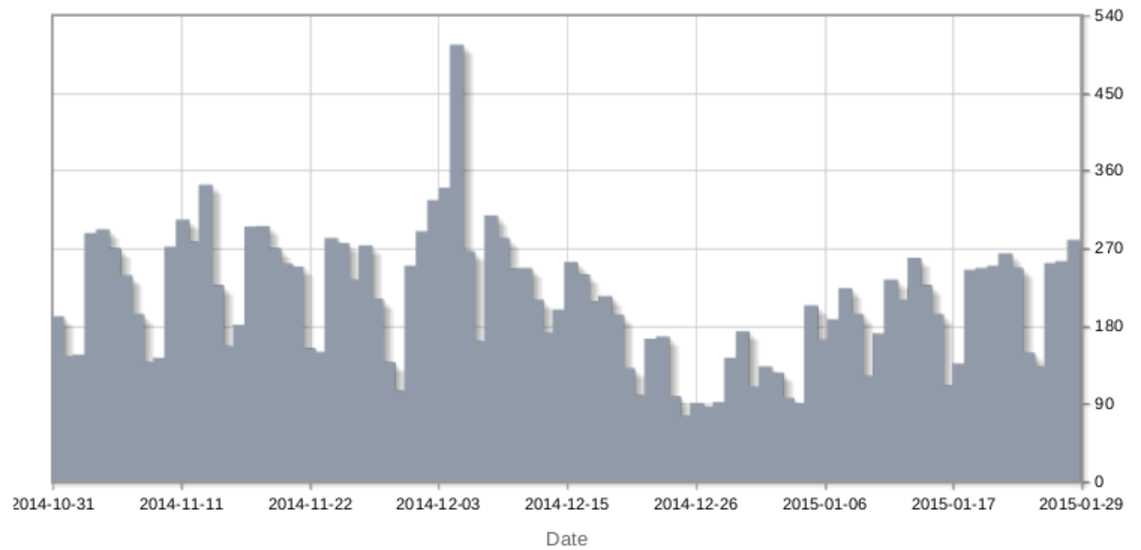
\includegraphics[width=\textwidth]{Abbildungen/wiki-spatialdatabase-usage.pdf}
\caption[Nutzungsstatistik der Wikipedia Seite spatial database]{Nutzungsstatistik von 90 Tagen der Wikipedia Seite \glqq Spatial database\grqq\ nach \cite{website:wiki-usage-spatialdatabase}}
\label{fig:wiki-usage-spatialdatabase}
\end{figure}
So wurde die Website am Mittwoch dem 21.1.2015 250 mal, dagegen am Samstag dem 17.1.2015 111 mal aufgerufen.
Allgemein ist an Tagen an Wochenenden etwa die Hälfte der Aufrufe pro Tag gegenüber Montag bis Freitag zu beobachten.
Weiterhin war zu den Weihnachtsfeiertagen eine wesentlich geringere Anzahl an Aufrufen zu verzeichnen: 1650 Aufrufe zwischen dem 22.12.2014 und 4.1.2015 im Gegensatz zu 3005 Aufrufe zwischen dem 8.12.2014 und 21.12.2014.
Diese Aufrufstatistik belegt das die Nutzung der Website etwa zur Hälfte durch Arbeitnehmer erfolgt und somit für Unternehmen interessant ist.

Schwer messbare Kriterien zur Softwareauswahl wie Marktposition, Support und Community fließen in diese Bewertung nicht ein, werden jedoch im Sinne der Agri Con ergänzend festgehalten.

\textbf{Auswahl eines Frameworks}\\
Aus der untersuchten Menge ist eines anhand der gemessenen Qualität auszuwählen.
Der Ist-Zustand\footnote{siehe \ref{IstStand}} der Agri Con ist über Jahre hinweg durch wachsende  Anforderungen im technischen und organisatorischen Bereich entstanden.
Aus diesem Grund ist die Auswahl eines Frameworks für den gesuchten Anwendungsfall aufwendig.
Die Wahrscheinlichkeit der Eignung mehrerer Frameworks scheint daher gering.
Dies ist eine subjektive Einschätzung des Autors, was es in dieser Teilaufgabe zu beweisen gilt.
Eine detaillierte Bewertung der Frameworks anhand aller Qualitäten würde danach dazu führen, dass kein Framework geeignet erscheint.
Deshalb ist die Auswahl eines Frameworks zunächst anhand deren Spezifikationen durchzuführen.

\textbf{Entwurf eines Prototypen}\\
Das ausgewählte Framework ist detailliert zu untersuchen.
Aus dieser Untersuchung soll ein Entwurf zum Einsatz bei der Agri Con entstehen.
Dabei ist besonders dessen Architektur zu beleuchten, eine Konfiguration zu erstellen und fehlende Funktionalitäten mit nachträglicher Implementierung in das Framework einzubinden.
Auf Grund der wesentlich unterschiedlichen Frameworks, kann vor der Auswahl keine konkrete Architekturempfehlung verwendet werden. Dieser Entwurf ist nach den Anforderungen und den Eigenheiten des Frameworks zu erstellen. Eine wesentliche Grundlage sind dabei Referenzimplementierungen und Guidelines des entsprechendem Rahmenwerkes.

\textbf{Prototypische Implementierung}\\
Der Entwurf wird schlussendlich umgesetzt und anhand der Metriken mit Funktions- und Leistungstests bewertet.
Auch diese Bewertung erfolgt im Rahmen einer Nutzwertanalyse, jedoch detaillierter.
Ziel ist dabei die Eignung des Prototypen hinsichtlich des geforderten Einsatzzweckes darzustellen.
Dafür werden die definierten Qualitäten herangezogen.
Außerdem soll eine Einschätzung aus Entwicklersicht gegeben werden, welche Preis, Marktposition, Support und Community einschätzt.
Diese Ergänzung ist notwendig, um weiterhin den Aufwand zur Einbindung des Frameworks in die Unternehmensstruktur und die Zukunftsfähigkeit einschätzen zu können.
% TODO: Bewertungsstruktur (Installation, ...) aufzählen und begründen

Für die grobe Nutzwertanalyse zur Auswahl eines Framworks ist im nachfolgenden Kapitel die Darstellung des Ist-Standes sowie die Anforderungen an das Framework zu finden.
Die Definition der Testfälle zur Datenerhebung für die detaillierte Nutzwertanalyse des Prototypen schließt sich daran an.